% Copyright 2004 by Till Tantau <tantau@users.sourceforge.net>.
%
% In principle, this file can be redistributed and/or modified under
% the terms of the GNU Public License, version 2.
%
% However, this file is supposed to be a template to be modified
% for your own needs. For this reason, if you use this file as a
% template and not specifically distribute it as part of a another
% package/program, I grant the extra permission to freely copy and
% modify this file as you see fit and even to delete this copyright
% notice. 

\documentclass{beamer}

\usetheme{Madrid}

\title[Sparse Noise]{Finding meaningful cluster structure \\ amidst background noise} % The short title appears at the bottom of every slide, the full title is only on the title page

\author[Shrinu Kushagra]
{%
  \texorpdfstring{
    \begin{columns}%[onlytextwidth]
      \column{.75\linewidth}
      \centering
      \vspace{25pt}\\ Shrinu Kushagra\\ \vspace{15pt}
      Oct 04, 2016 \\ \vspace{15pt}
      Joint work with Samira Samadi and Shai Ben-David
    \end{columns}
    \vspace{5pt}
	  \begin{figure}
	  
\includegraphics[trim = 0 50 0 0, clip, width=0.3\linewidth]{logo.pdf}
	  \end{figure}  
  }
  {}
}


\AtBeginSubsection[]
{
  \begin{frame}<beamer>
  \frametitle{Outline}
    \tableofcontents[currentsection]
  \end{frame}
}

\newcommand{\mc}{\mathcal}

% Let's get started
\begin{document}

\begin{frame}
  \titlepage
\end{frame}

\begin{frame}{Outline}
  \tableofcontents
  % You might wish to add the option [pausesections]
\end{frame}

% Section and subsections will appear in the presentation overview
% and table of contents.
\section{Introduction}

\begin{frame}{Clustering - Introduction}
  Input: A list of objects $\mc X$ and the number of clusters $k$\\
  Output: A  clustering (partition) $\mc C$ of the set $\mc X$. That is, $\mc C = \{X_1, \ldots, X_k\}$\\
  
  \pause
  \vspace{0.1in} Most common approach
  \begin{itemize}
  	\item Associate a cost with each possible clustering $\mc C$.
  	\item Find the clustering with minimum cost. $$\min_{\mc C} \sum_{i=1}^k \sum_{x \in X_i} \|x - \mu(X_i)\|^2$$
  \end{itemize}
\end{frame}

\begin{frame}{Clustering - Challenges}  
  Computationally expensive\\
  \begin{itemize}
  	\item Minimizing objective is NP-Hard.
  	\item Approximating is also hard.
  \end{itemize}
  \vspace{0.1in}Multiple solutions
  \begin{itemize}
  	\item Same set can be clustered in multiple ways.
  	\item Different clusterings depending upon application.
  \end{itemize}
\end{frame}


\begin{frame}{Clustering is difficult only when it doesnt matter}
  
  Theory vs Practice
  \begin{itemize}
	\item Theory says not possible to find ``optimal clustering''.
  	\item In practice, $K$-Means is used.
  	\item Successful on various tasks.
  \end{itemize}
  
  \vspace{0.2in}Possible explanation/solution.
  \begin{itemize}  
  	\item Real world data sets have some nice structure.
  	\item Clustering is easy (computationally) if the input has this nice structure. 
  	\item Formalize ``data is well-separated'' assumption.
  \end{itemize}
\end{frame}

\begin{frame}{Notions of clusterability}
  \begin{itemize}
  	\item $\alpha$-center proximity\\
    A clustering $\mc C$ satisfies $\alpha$-center proximity w.r.t $\mc X$ if there exist centers $c_1, \ldots, c_k$  such that the following holds. For all $x \in X_i$ and $i\neq j$, $$\alpha d(x, c_i) < d(x, c_j)$$ 
  	\item $\lambda$-center separation\\
  	A clustering $\mc C$ has $\lambda$-center separation w.r.t $\mc X$ if there exists centers $c_1, \ldots, c_k$ such that the following holds. For all $i\neq j$, 
  	$$d(c_i, c_j) > \lambda r(\mc C)$$
  \end{itemize}
\end{frame}

\section{Previous Work}

\begin{frame}{Known Results}
  Intuition
  \begin{itemize}
    \item $\alpha$ controls how separated the clusters are.
    \item Bigger the $\alpha$, more the separation.  
  \end{itemize}
  
  \vspace{0.2in}Goal: Find the optimal $k$-median solution. It is known that the optimal solution satisfies $\alpha$-center proximity. 
  \begin{itemize}
    \item $\alpha > \sqrt{2}+1$ - Efficient algorithm based on finding a $k$-pruning of a hierarchical clustering tree.
    \item $\alpha < 2$ - Problem NP-Hard.  
  \end{itemize}
\end{frame}

\begin{frame}{Known results}
	Limitations
	\begin{itemize}
		\item Assumes entire set $\mc X$ has a nice structure.
		\item Too strict. Unrealistic in pratical situations.
	\end{itemize}
	\vspace{0.1in}Solution
	\begin{itemize}
		\item Noise - Add points which do not have any structure
	\end{itemize}
	\vspace{0.2in}Goal: Find the optimal $k$-median solution. It is known that the optimal solution satisfies $\alpha$-center proximity except for an $\epsilon$ fraction of points. 
  \begin{itemize}
    \item $\alpha > 2+\sqrt{7} \approx 4.6$ - Efficient algorithm  finds a $1+O(\epsilon)$ approximation to $k$-median optimal.
  \end{itemize}
\end{frame}

\section{Big Picture}

\begin{frame}{Problem Setting}
  Limitations
  \begin{itemize}
  	\item Impossible to verify - Can't find optimal solution. No way to verify if the optimal has that property.
  	\item Small noise - Upper bounded by a fraction of the dataset.  
  \end{itemize}
  \vspace{0.2in}Our framework
  \begin{itemize}
  	\item Noise is structureless.
  	\item Efficient representation of all nice solutions.
  \end{itemize}
\end{frame}

\begin{frame}{Contributions}
  Results under $\alpha$-center proximity\\
  \begin{itemize}
  	\item $\alpha < 3 + 2\sqrt{2} \approx 5.8$ and noise is small - No efficient representation exists. 
  	\item $\alpha > 2 + \sqrt{7} \approx 4.6$ and noise is sparse - Efficient algorithm which captures all solutions.
  	\item $\alpha < 3 + \sqrt{2} \approx 4.4$ and noise is sparse - No efficient representation exists.
  \end{itemize}
\end{frame}

\begin{frame}{Contributions}
  Results under $\lambda$-center separation\\
 \begin{itemize}
  	\item $\lambda < 6$ and noise is small - No efficient representation exists. 
  	\item $\lambda > 4$ and noise is sparse - Efficient algorithm which captures all solutions.
  	\item $\lambda < 4$ and noise is sparse - No efficient representation exists.
  \end{itemize}
  \vspace{0.2in}Structureless noise is natural.
\end{frame}

\section{Preliminaries}

\begin{frame}{Definitions}
	Given a clustering $\mc C = \{C_1, \ldots, C_k\}$ induced by centers $c_1, \ldots, c_k$, $m(\mc{C}) = \min_i |C_i|$ and $r(\mc{C}) = \max_i \thinspace r(C_i)$.
	
	\vspace{0.1in}\begin{block}{($\alpha, \eta$)-center proximity}
	Given $\mc S \subseteq \mc X$, a clustering $\mc C_{\mc S} = \{S_1, \ldots, S_k\}$ has $(\alpha, \eta)$-center proximity if there exists centers $s_1, \ldots, s_k$  such that the following holds.
	\begin{itemize}
  	\item[$\diamond$] {\bf $\alpha$-center proximity}: For all $x \in S_i$ and $i\neq j$, $\thinspace\alpha d(x, s_i) < d(x, s_j)$
	\item[$\diamond$]{\bf $\eta$-sparse noise}: For any ball $B$, $r(B)\leq \eta \thinspace r(\mc{C}_{\mc S}) \implies |B\cap (\mc X\setminus \mc S)| < \frac{m(\mc C_{\mc S})}{2}$
	\end{itemize}
	\end{block}
\end{frame}

\begin{frame}{Definitions}
	Given a clustering $\mc C = \{C_1, \ldots, C_k\}$ induced by centers $c_1, \ldots, c_k$, $m(\mc{C}) = \min_i |C_i|$ and $r(\mc{C}) = \max_i \thinspace r(C_i)$.

	\vspace{0.1in}\begin{block}{($\lambda, \eta$)-center separation}
	Given $\mc S \subseteq \mc X$, a clustering $\mc C_{\mc S}$ has $(\lambda, \eta)$-center separation if there exists centers $s_1, \ldots, s_k$ such that $\mc C_{\mc X}$ is the clustering induced by these centers and the following holds.

	\begin{itemize}
	\label{defn:lambdacsnoise}	

	\item[$\diamond$] {\bf $\lambda$-center separation}: For all $i\neq j$, $\thinspace d(s_i, s_j) > \lambda r({\mc C}_{\mc S})$
	\item[$\diamond$]{\bf $\eta$-sparse noise}: For any ball $B$, $r(B)\leq \eta \thinspace r(\mc{C}_{\mc S}) \implies |B\cap (\mc X\setminus \mc S)| < \frac{m(\mc C_{\mc S})}{2}$
	\end{itemize}
	\end{block}
\end{frame}

\section{Algorithmic Approach}


\begin{frame}{Clustering under $\alpha$-center proximity}
	\begin{block}{The algorithm}
	  Input: $(\mc X, d)$ and a parameter $t$.\\
	  Output: A hierarchical clustering tree.\\
	  \vspace{0.1in}Initialize every point in its own cluster.\\
	  Go over all pairs of points $p, q$ in increasing order of distance.\\
	  If $B := B(p, d(p, q))$ satisfies the sparse-distance condition
	  \begin{itemize}
	  	\item Merge all clusters that intersect with $B$ into a single cluster
	  \end{itemize}
    \end{block}
        
    \vspace{0.2in}We say that the ball $B$ satisfies the sparse distance condition w.r.t clustering $\mc C$ when the following holds.
	\begin{itemize}
	  \item $|B| \ge t$.
	  \item For any $X_i \in \mc C$, if $X_i \cap B \neq \emptyset$, then $X_i \subseteq B$ or $|B \cap X_i| \ge t/2$.
	\end{itemize}
\end{frame}

\begin{frame}{Clustering under $\alpha$-center proximity}
	\begin{block}{Proof Idea}
	\begin{itemize}
	  \item Let the target clustering be $\mc C^* = \{S_1^*, \ldots, S_k^*\}$
	  \item If points from $S_i^*$ is merged with points from $S_j^*$,  then at this step the distance being considered $d = d(p,q) > r(S_i^*)$.	
      \item When the algorithm considers the distance $d = r(S_i^*)$, it merges all points from $S_i^*$ into a single cluster. 
    \end{itemize} 	
	\end{block}
\end{frame}

\begin{frame}{Clustering under $\alpha$-center proximity}
	\begin{block}{Result}
	\begin{itemize}
	  \item Given a clustering instance $(\mc X, d)$ and a parameter $t$. outputs a tree $\mc T$ with the following property. For all $k$, $\mc S \subseteq \mc X$ and for all $k$-clusterings $\mc C^*_{\mc S} = \{S_1^*, \ldots, S_k^*\}$ which satisfy $(2+\sqrt{7}, 1)$-center proximity the following holds. If $m(\mc C_{\mc S}^*) = t$ then $\mc T$ captures $\mc C_{\mc S}$.
	  \item Runs in polynomial time.
	\end{itemize}
	\end{block}
\end{frame}

\begin{frame}{Clustering under $\alpha$-center proximity}
	If $\alpha < 3 + \sqrt{2}$ and noise is sparse, then there doesn't exist a clustering tree which can capture all nice solutions.
	\begin{figure}[!t]
	  \begin{center}
	    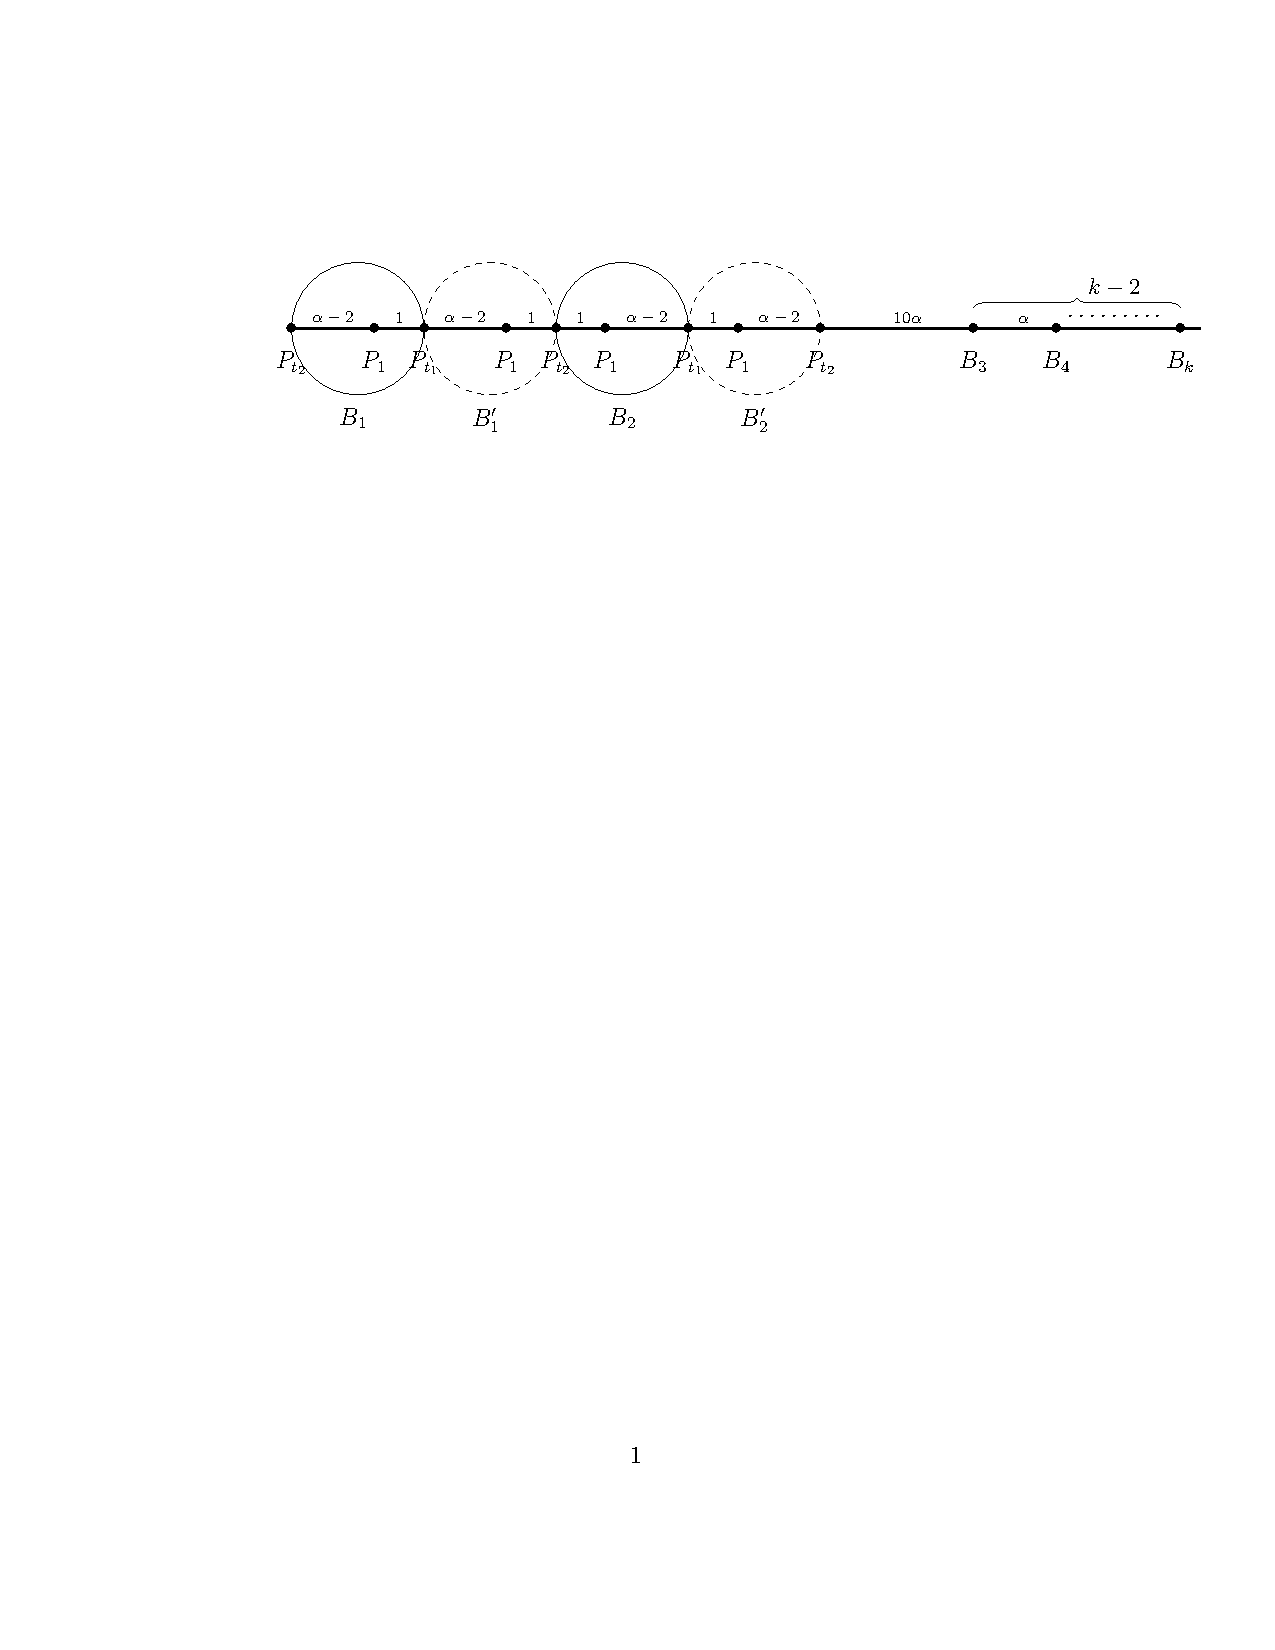
\includegraphics[trim={47mm 205mm 12mm 44mm},clip,width=\textwidth]{lbdFig2.pdf}
	  \end{center}
	\end{figure}
	Same ideas can be extended to a list output. Any list should have size $> 2^{k/2}$
\end{frame}

\begin{frame}{Clustering under $\alpha$-center proximity}
	If $\alpha < 3 + 2\sqrt{2}$ and noise is arbitrary, then there doesn't exist a clustering tree which can capture all nice solutions.
	\begin{figure}[!t]
	  \begin{center}
	    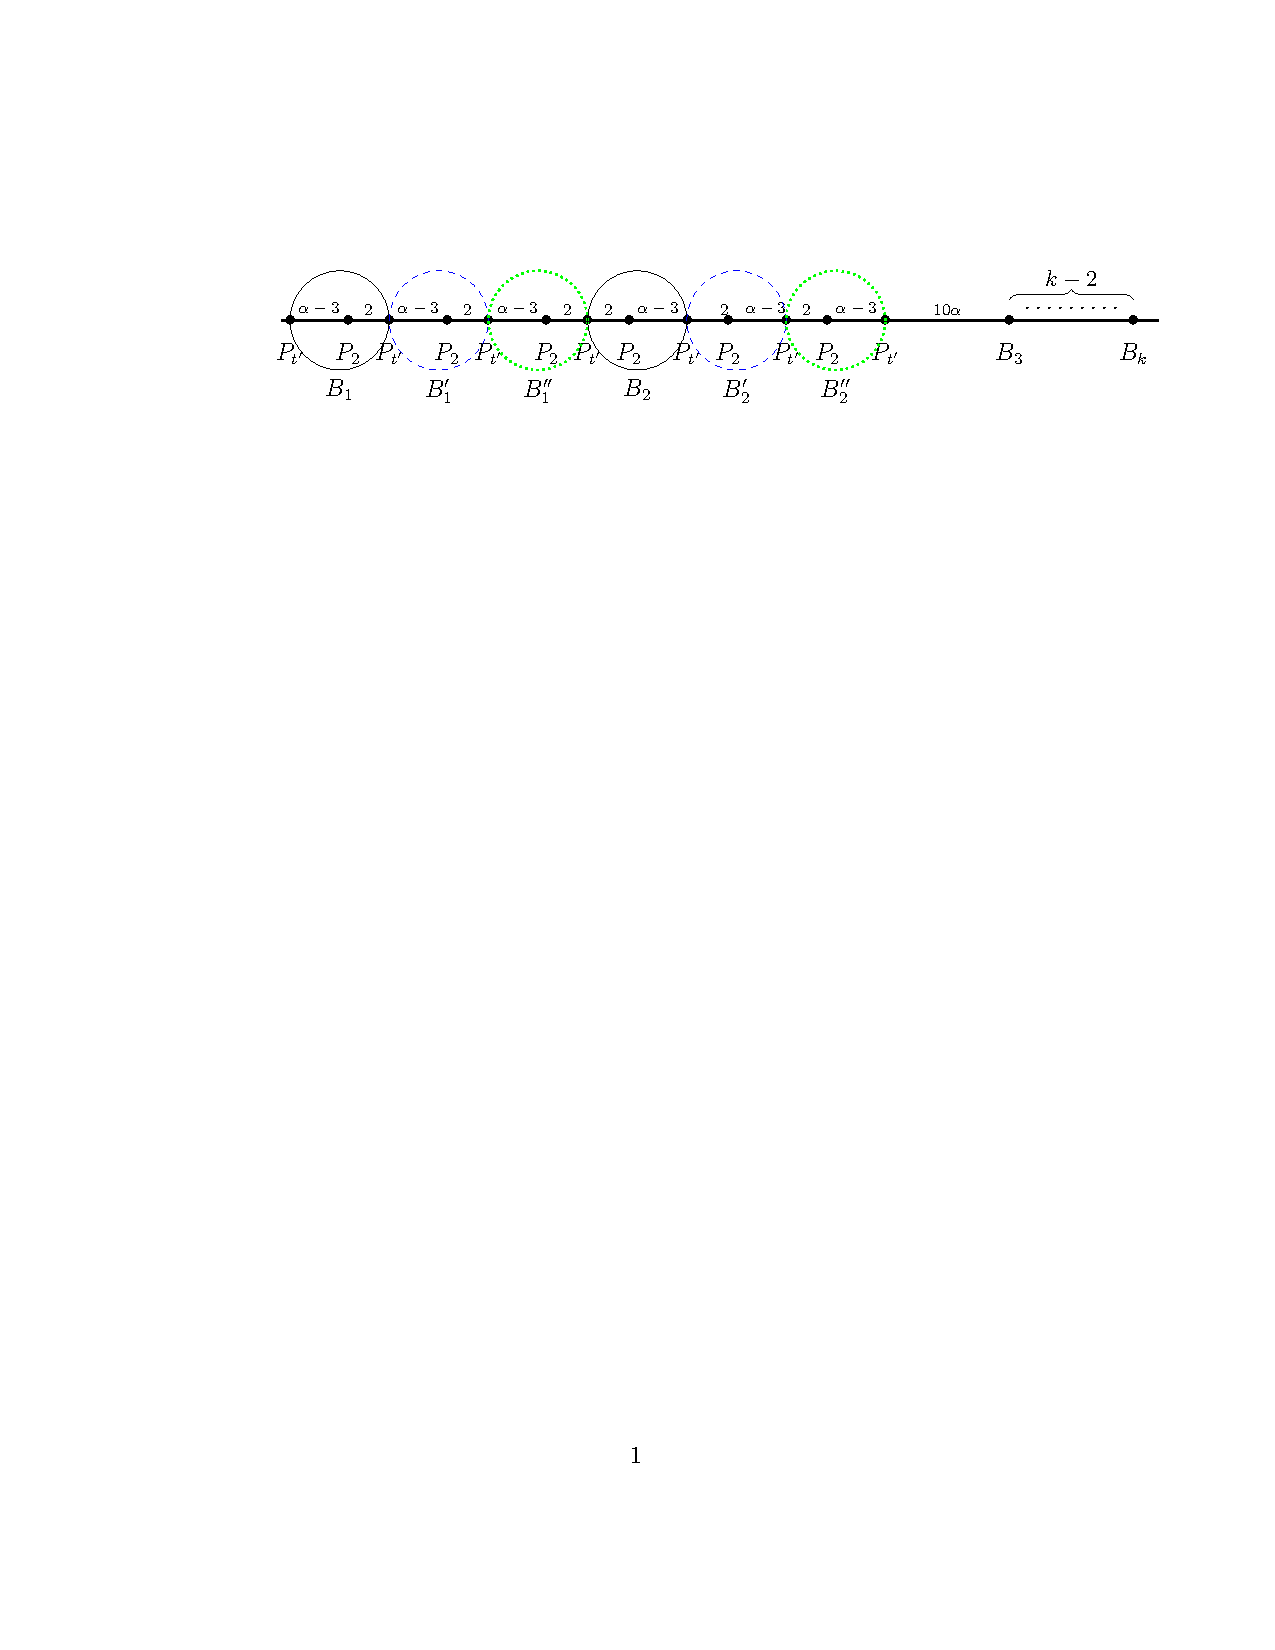
\includegraphics[trim={47mm 205mm 12mm 44mm},clip,width=\textwidth]{lbdFig3.pdf}
	  \end{center}
	\end{figure}
	Same ideas can be extended to a list output. Any list should have size $> 2^{k/2}$
\end{frame}

\begin{frame}{Clustering under $\lambda$-center separation}
	\begin{block}{The algorithm}
	  Input: $(\mc X, d)$ and parameters $r$ and $t$.\\
	  Output: A clustering of $\mc X$.\\
	  \vspace{0.1in}Initialize every point in its own cluster.\\
	  Construct a list $L$ of balls $B$ such that $r(B) \le r$ and $m(B) \ge t$.\\
	  Construct a vertex in a graph for every ball in the list. \\
	  If $B_i \cap B_j \ge t/2$, connect the vertices by an edge.\\
	  Output the connected components as a clustering of the set.
    \end{block}
\end{frame}

\begin{frame}{Clustering under $\lambda$-center separation}
	\begin{block}{Proof Idea}
	\begin{itemize}
	  \item Let the target clustering be $\mc C^* = \{S_1^*, \ldots, S_k^*\}$
	  \item If $B_{i1}$ and $B_{i2}$ intersect $S_i^*$ then the vertices $v_{i1}$ and $v_{i2}$ are connected.
	  \item If $B_{i1}$ intersects $S_i^*$ and $B_{j1}$ intersects $S_j^*$ then $v_{i1}$ and $v_{j1}$ are disconnected in $G$.	
    \end{itemize} 	
	\end{block}
\end{frame}

\begin{frame}{Clustering under $\lambda$-center separation}
	\begin{block}{Result}
	\begin{itemize}
	  \item Given a clustering instance $(\mc X, d)$ and parameters $r$ and $t$. For every $k$, for every $\mc S \subseteq \mc X$ and for all $k$-clusterings $\mc C^* = \{S_1^*, \ldots, S_k^*\}$ which satisfy $(4, 1)$-center separation such that $ m(\mc C_{\mc S}^*) = t$ and $r(\mc C_{\mc S}^*) = r$, the following holds. Alg. outputs a clustering $\mc C$ such that $\mc C|_{\mc S} = \mc C_{\mc S}^*$.
	  \item Runs in polynomial time.
	\end{itemize}
	\end{block}
	The lower bounds are obtained using identical techniques as the lower bounds for $\alpha$-center proximity case.
\end{frame}

\begin{frame}{Sparse noise is natural}
    \begin{itemize}
	  \item Let data $\mc S$ has nice structure (cohesive and separated sets).
	  \item Uniform random noise $\mc N$ is added to this data.
	  \item $\mc X = \mc S \cup \mc N$ satisfies the structureless noise definition with high probability.
    \end{itemize}
\end{frame}

\begin{frame}
    \Huge{\centerline{Thank You!}}
\end{frame}

%----------------------------------------
%        Figure Samples
%----------------------------------------

% All of the following is optional and typically not needed. 
\appendix
\section<presentation>*{\appendixname}
\subsection<presentation>*{For Further Reading}

%\begin{frame}[allowframebreaks]
  %\frametitle<presentation>{For Further Reading}
   % 
  %\begin{thebibliography}{10}
    
  %\beamertemplatebookbibitems
  % Start with overview books.

  %\bibitem{Author1990}
   % A.~Author.
    %\newblock {\em Handbook of Everything}.
    %\newblock Some Press, 1990.
 
    
  %\beamertemplatearticlebibitems
  % Followed by interesting articles. Keep the list short. 

  %\bibitem{Someone2000}
   % S.~Someone.
    %\newblock On this and that.
    %\newblock {\em Journal of This and That}, 2(1):50--100,
    %2000.
  %\end{thebibliography}
%\end{frame}

\end{document}


